% !TEX root = ../Noctua_Pflichtenheft.tex

\chapter{Projektplanung}
\label{chapter:Projektplanung}

\section{Projektstrukturplan}

\begin{minipage}[t]{\textwidth}
{\centering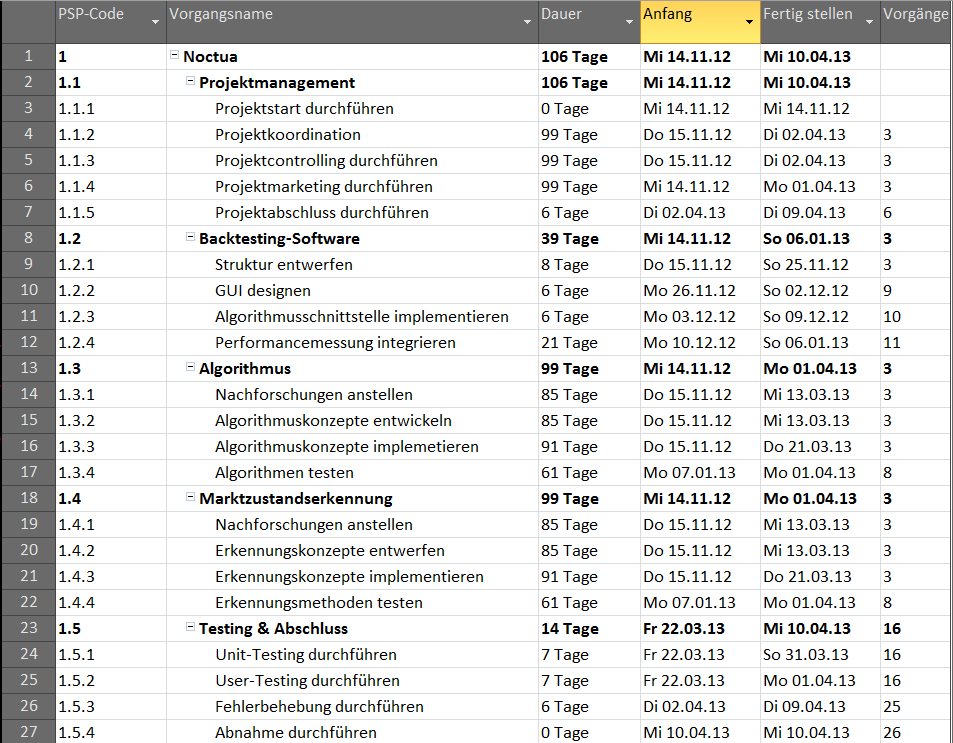
\includegraphics[width=1.00\textwidth]{graphics/projektplanung/psp.png}
\captionof{figure}{Projektstrukturplan}}
\end{minipage}

\section{Balkenplan}

\begin{minipage}[t]{\textwidth}
{\centering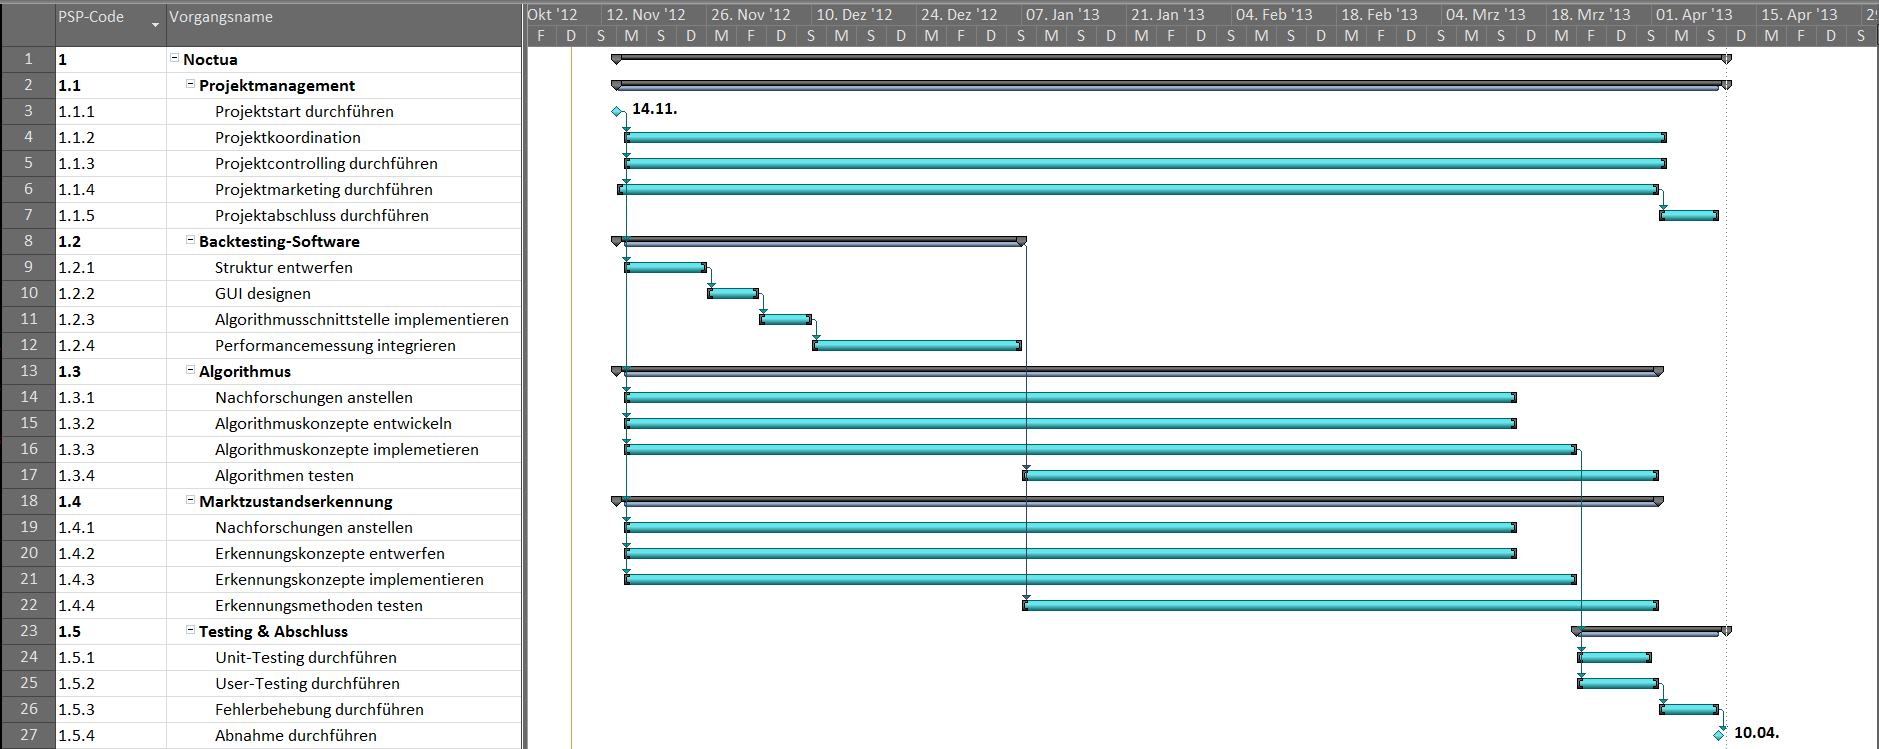
\includegraphics[width=1.00\textwidth]{graphics/projektplanung/balkenplan.png}
\captionof{figure}{Balkenplan}}
\end{minipage}

\section{Meilensteinplan}

\begin{center}

\begin{tabular}{ | p{3.5cm} | p{7.5cm} | l |}
\hline 
\textbf{Meilenstein}�& \textbf{Deliverable} & \textbf{Datum}\\  \hline
Projektstart & ~ & 14.11.2012 \\  \hline
\gls{bts} fertiggestellt & \gls{bts} + dazugeh�rige Dokumentation & 06.01.2013 \\ \hline
Produkt fertiggestellt & Version des Produkts (\gls{bts} + Algorithmus), die noch nicht getestet wurde die dazugeh�rige Dokumentation & 21.03.2013 \\ \hline
Testing abgeschlossen & Testberichte und etwaige Verbesserungen am Produkt & 09.04.2013 \\ \hline
Projektabnahme & Ausgef�lltes Abnahmeprotokoll & 10.04.2013 \\ \hline

\end{tabular}

\end{center}